\chapter{Requirement Analysis}
  Up to now AutoWDS automatically uses just one or a random set of channels for its backbone wireless connections. 
  Additionally the topology it creates often reassembles a tree like structure, since the APs connect themselves 
  to the first AP that comes into range and there is no fallback, if a link fails. This results not only in huge bottlenecks for throughput,
  it also leads to greater downtimes if a link happens to fail. Although the APs automatically rejoin the network if possible, it takes
  a considerable amount of time until they are fully reconnected. This is somehow undesirable for the Systems that use this AP as an uplink connection to
  the network. The following requirements for an improved Version of AutoWDS are supposed to tackle those shortcomings.
  \begin{figure}[t]
    \centering
    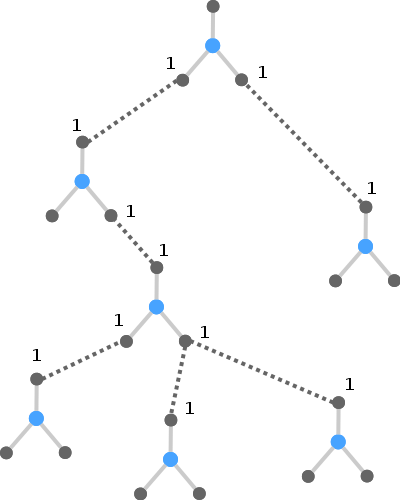
\includegraphics[width=0.3\columnwidth]{figures/autowds_basic_graph}
    \caption{AutoWDS basic network topology and channel assignment}
    \label{fig:autowds_basic_graph}
  \end{figure}
General answer to question of feasibility
  \section{Increase Throughput}
  Since the systems which are connected to the accesspoints consume more data every day and with an increasing storage-footprint of new media like streaming HD videos
  and generally downloading files of up to Gigabytes, a Wireless system is often solely defined by its capability shoveling data over the air to the clients.
  This greed for throughput is amplified by an increasing number of devices that take part in radio communication, 
  thus it is also the key metric for quality in AutoWDS. Furthermore not a single stream of data should be granted exclusively access to the radio, but
  many streams in parallel are desired.
  \section{Reduce Network Connectivity Failures}
\section{Utilize variable Number of Radios}
  Should utilize multiple Radios per AP\newline
  Currently homogenous 2, Later 3, sometimes just 1 \newline
  Also should be able to handle heterogenous environments with respect to number of equipped radios \newline
  \section{Capability of using variable channels}
  Not just fixed amount, but depending on the usecase, like: only 1 and 11 or only 36,40,44
  \section{Restrictions}
  \subsection{Centralized Computation}
    Run on central entity (WLC), not distributed \newline 
  \subsection{Static Environment}
    System is only used for static environments (APs are not mobile) \newline
\section{Economical Restrictions}
  Ressource restrictions (Processing Power limited) \newline
  Duration (Results have to be available in limited time) \newline
